\documentclass[a4paper,16pt]{article}
\usepackage[a4paper, total={6in, 8in}]{geometry}

\usepackage{euscript}
\usepackage[utf8]{inputenc}
\usepackage[english,ukrainian]{babel}
\usepackage{mathtext}
\usepackage{epigraph}
\usepackage{indentfirst}
\usepackage{graphicx}
\usepackage{amsmath, amsthm,amsfonts,amsmath,amssymb,amscd}
\usepackage{mathrsfs}
\usepackage{apacite}
\usepackage{tabularx}
\usepackage{tikz}
\usepackage{hyperref}

\usepackage{longtable,booktabs}
\usepackage{stmaryrd}

\graphicspath{{images/}}
\DeclareGraphicsExtensions{.png,.jpg}

% ************************************************************* %
%  Визначення математичних оточень та роботи з формулами
% ************************************************************* %

\theoremstyle{plain}
\newtheorem{theorem}{\indent Теорема}[chapter]
\newtheorem{claim}{\indent Твердження}[chapter]
\newtheorem{lemma}{\indent Лема}[chapter]	
\newtheorem{corollary}{\indent Наслідок}[chapter]

\theoremstyle{definition}
\newtheorem{definition}{\indent Означення}[chapter]
\newtheorem{algorithm}{\indent Алгоритм}[chapter]
\newtheorem{problem}{\indent Задача}[chapter]
\newtheorem{example}{\indent Приклад}[chapter]
\theoremstyle{remark}
\newtheorem*{remark}{\indent\textbf{Зауваження}}
\renewenvironment{proof}{{\indent\bfseries Доведення.~}}{\qed}

% змінюємо формат нумерації формул
\renewcommand{\theequation}{\arabic{chapter}.\arabic{equation}}

% команди для заборони розриву формул у небажаному місці
\binoppenalty=10000
\relpenalty=10000


% ************************************************************* %
%  Ненумеровані розділи
% ************************************************************* %

% команда для створення ненумерованого розділу, який тим не менше показується в змісті
\newcommand{\uchapter}[1]{\chapter*{#1}\addcontentsline{toc}{chapter}{#1}} 

\newcommand{\intro}{\uchapter{Вступ}}                   % для створення вступу використаємо команду \uchapter
\newcommand{\conclusions}{\uchapter{Висновки}}          % для створення висновків використаємо команду \uchapter
\newcommand{\shortings}{\uchapter{Перелік умовних позначень, скорочень і термінів}}
                                                        % для створення переліку умовних позначень використаємо команду \shortings

\newcommand{\chapconclude}[1]{\section*{Висновки до розділу #1} \addcontentsline{toc}{section}{Висновки до розділу #1}}

\def\checkmark{\tikz\fill[scale=0.4](0,.35) -- (.25,0) -- (1,.7) -- (.25,.15) -- cycle;} 

%основний документ
\begin{document}


% Титульный лист
	\thispagestyle{empty}
	
	\begin{center}
		НАЦІОНАЛЬНИЙ ТЕХНІЧНИЙ УНІВЕРСИТЕТ УКРАЇНИ \par
		<<КИЇВСЬКИЙ ПОЛІТЕХНІЧНИЙ ІНСТИТУТ ім. Ігоря СІКОРСЬКОГО>>\par
		НАВЧАЛЬНО-НАКУОВИЙ ФІЗИКО-ТЕХНІЧНИЙ ІНСТИТУТ\par
		
		\vspace{60mm}
		{\huge Звіт за темою:\par
			\LARGE <<Дослідження алгоритмів реалізації арифметичних операцій
			 над великими числами>>\par}
		
	\end{center}
	
	\vspace{40mm}
	\begin{flushright}
		Виконали студенти
		
		групи ФІ-32мн
		
		Баєвський Констянтин,
		
		Шифрін Денис,
		
		Кріпака Ілля
		
	\end{flushright}
	
	\vspace{27mm}
	\begin{center}
		{Київ~--- 2023}
	\end{center}
	

\newpage

\pagenumbering{gobble}
\cleardoublepage
\pagenumbering{arabic}

\setcounter{page}{2} 

\section{Мета практикуму}

Дослідити алгоритми реалізації готових бібліотек над великими числами, скінченними полями та групами із точки зору ефективності за часом та пам'яттю.

\subsection{Постановка задачі та варіант}
\begin{tabularx}{\textwidth}{X|X}
	\textbf{Треба виконати} & \textbf{Зроблено} \\
	Дослідити бібліотеки на мові Rust & \checkmark \\
	Дослідити бібліотеки на мові C# & \checkmark \\
	Дослідити бібліотеки на мові Python? & \checkmark \\
\end{tabularx}

\section{Хід роботи/Опис труднощів}
	На початку роботи гуртом вибрали варіант 1С та мови на яких будемо проводити дослідження -- Rust, C#, Python?. Також у нас виникала лише одна часова складність :-).

\section{Результати дослідження}
На початку доcлідження варто зазначити, що, відповідно до нашого досвіду, можна побачити в основному бібліотеки створються трьома способами:
\begin{enumerate}
	\item реалізуються на мовах C/C++ і використовується там же;
	\item реалізуються тою мовою, де їх будуть використовувати (до прикладу, крейт \href{https://docs.rs/crypto-bigint/latest/crypto_bigint/}{crypto-bigint} у Rust);
	\item спочатку реалізуються як із пункту 1, а потім пишеться певна обгортка над операціями/типами задля легкості використання.
\end{enumerate}

Спробуємо провести аналіз деяких із представників цих бібліотек.

\subsection{С/С++ бібліотеки}
Спочатку наведемо короткий опис із бібіліотек, що можна було взяти до аналізу прямо із завдання лабораторної роботи. Потрібно одразу попередити, що поки для нас C/C++ дається туго(.

\begin{itemize}
	\item Pari/GP -- спеціалізована комп'ютерна алгебраїчна система, що у більшості використовується науковцями для різних областей від топології чи числового аналізу до фізики. Як зрозуміли, то GP у ній є такою собі спеціалізованою скриптовою мовою, а PARI, що є безпосередньо \href{https://pari.math.u-bordeaux.fr/pub/pari/manuals/2.7.6/libpari.pdf}{libpari} бібліотекою написаною на С.
		
	\begin{figure}[h]
    		\centering
    		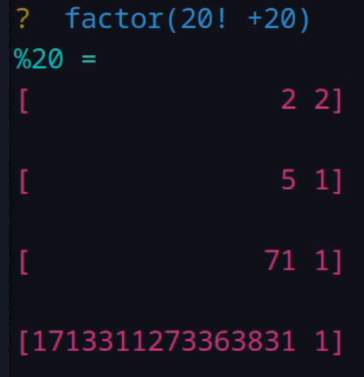
\includegraphics[scale = 0.25]{Images/pari_gp}
    		\caption{Приклад факторизації числа $20! + 20$ на мові GP.}
    		\label{fig:}
	\end{figure}

	
	\item GNU GMP -- безкоштовна бібліотека для арифметики довільної точності, яка працює над цілими числами зі знаком, раціональними числами та числами з плаваючою комою. Тут немає жодних практичних обмежень точності, окрім тих, що передбачають доступну пам’ять у машині, на якій працює GMP. GMP  має багатий набір функцій, і функції мають звичайний інтерфейс.
	
	\begin{figure}[h]
    		\centering
    		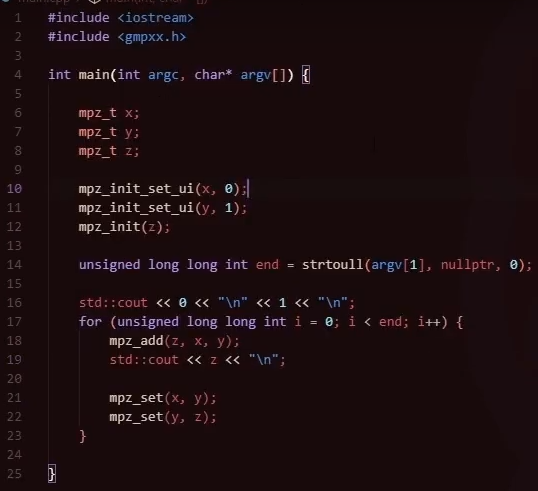
\includegraphics[scale = 0.25]{Images/gnu_gmp}
    		\caption{Приклад виводу у циклі підсумованих великих чисел із використанням  типів GNU GMP бібліотеки.}
    		\label{fig:}
	\end{figure}
\end{itemize}

\subsection{Обгортки над С/С++}

\begin{itemize}
	\item \href{https://crates.io/crates/rug}{Rug} надає цілі числа та числа з плаваючою комою з довільною точністю та округленням разом із операціями над ними. Саме ця бібліотека реалізовує високорівневий інтерфейс над бібліотеками GNU:
	\begin{itemize}
		\item GMP (для цілих чисел та раціональних чисел),
		\item MPFR (для чисел із плаваючою точкою),
		\item MPC (для комплексних чисел).
	\end{itemize}
		
	Надалі наведу трохи скрішотів та пояснень до коду для цілочисельного типу.
	
	Почнемо із піднесення до степеня.
	\begin{figure}[h]
    		\centering
    		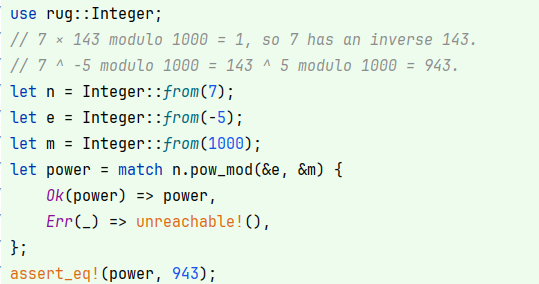
\includegraphics[scale = 0.25]{Images/pow_mod_rug}
    		\caption{Приклад використання піднесення до степеня за модулем.}
    		\label{fig:pow_mod_rug}
	\end{figure}
	
	\begin{figure}[h]
    		\centering
    		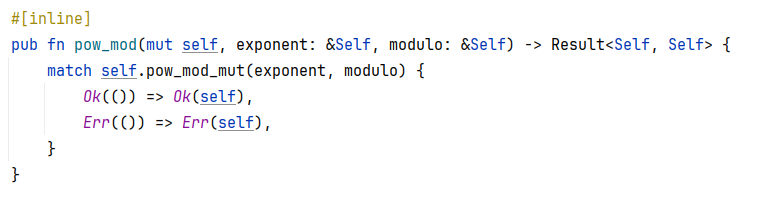
\includegraphics[scale = 0.25]{Images/pow_mod_rug_code1}
    		\caption{Код який використовує функція \ref{fig:pow_mod_rug}.}
    		\label{fig:pow_mod_rug_code1}
	\end{figure}
	
	\begin{figure}[h]
    		\centering
    		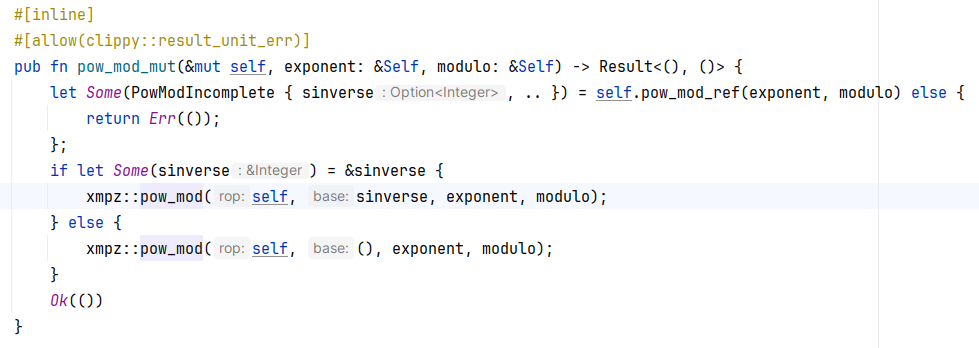
\includegraphics[scale = 0.25]{Images/pow_mod_rug_code2}
    		\caption{Далі функція \ref{fig:pow_mod_rug_code1} переходить сюди.}
    		\label{fig:pow_mod_rug_code2}
	\end{figure}	
	
	\begin{figure}[h]
    		\centering
    		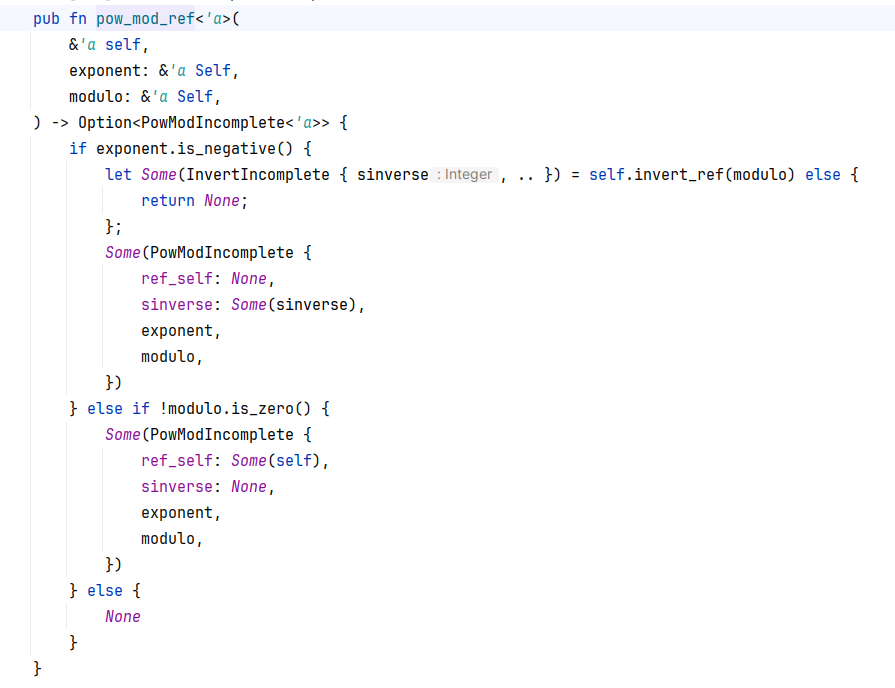
\includegraphics[scale = 0.25]{Images/pow_mod_rug_safe}
    		\caption{За умови збереженого значення переходимо у цю функцію із \ref{fig:pow_mod_rug_code2}.}
    		\label{fig:pow_mod_rug_safe}
	\end{figure}	
	
	\begin{figure}[h]
    		\centering
    		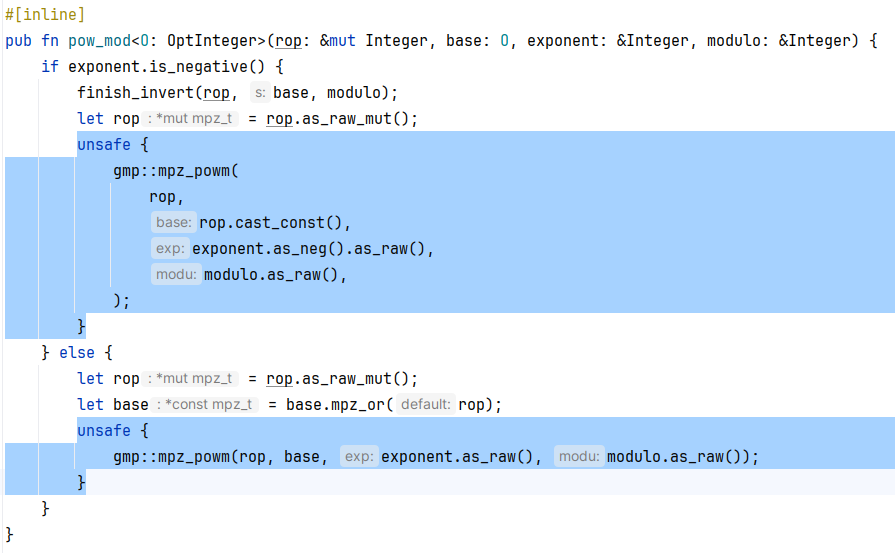
\includegraphics[scale = 0.25]{Images/pow_mod_rug_unsafe}
    		\caption{Задля обчислення числа заново, переходимо сюди із \ref{fig:pow_mod_rug_code2}.}
    		\label{fig:pow_mod_rug_unsafe}
	\end{figure}
	
	Тепер пояснимо код піднесення до степеня. Перший скріншот \ref{fig:pow_mod_rug} є прикладом до використання. Потім як передемо по коду, передемо до скріншоту \ref{fig:pow_mod_rug_code1} -- це є відправною точкою. Далі від неї переходимо у функцію \ref{fig:pow_mod_rug_code2}. Вона має у собі розвилку, \ref{fig:pow_mod_rug_safe} переходить і повертає збережені значення як такі є, а \ref{fig:pow_mod_rug_unsafe} спускається до виклику функції із C. Усе це можливо завдяки FFI(Foreign Funciton Interface), що є певним механізмом, де програма написана на одній мові програмування може використовувати бібліотеки/сервіси написані на іншій мові програмування. У Rust FFI забезпечує абстракцію без витрат, що зводиться до швидкості виконання коду на C. Наведемо ще один приклад функції.
	
	Цього разу будемо викликати
	
	
	\item С#??
\end{itemize}

\subsection{Нативні бібліотеки}





\begin{figure}[h]
    \centering
    \includegraphics[scale = 0.25]{Images/conditional_prob}
    \caption{Таблиця умовних ймовірностей для обчислення вирішуючих функцій.}
    \label{fig:twisted_edward}
\end{figure}















\section{Висновки}
За допомогою реалізації практикуму ''Баєсiвський пiдхiд в криптоаналiзi: побудова i дослiдження детермiнiстичної та стохастичної вирiшуючих функцiй'' дізналися на практиці як повинен відбуватися баєсівський підхід у криптоаналізі. Також були долучені до створення такого собі <<маленького>> прикладу із побудови вирішуючих функцій для заданого розподілу повідомлень.


\end{document}

